\chapter{Revisão Bibliográfica} \label{capitulo1}
%label cria um rótulo para o objeto, para permitir que ele seja referenciado com o comando \ref{nome-do-rotulo}

\section{Objetivos da 5G} 
" O desenvolvimento da sociedade vai levar a mudanças na forma como os sistemas de comunicação sem-fio e móveis são usados". É assim que Afif Osseiran, diretor do departamento de comunicação por rádio da Ericsson inicia o resumo de seu artigo "Scenarios for 5G mobile and wireless communications: the vision of the METIS project" \cite{Afif}. 
\par Para possibilitar essas mudanças, formaram-se alguns grupos e projetos, tais como o europeu METIS \cite{Roh}, e o chinês IMT-2020. Nesse contexto, especificou-se em quais cenários estaria empregado o 5G. Definiram-se 5 \cite{Afif}:
\begin{itemize}
\item \textbf{\textit{"Amazingly Fast"}} - traduzido como "incrivelmente rápido", foca na transmissão de dados em alta velocidade 
\item \textbf{"Ótimo serviço na multidão"} - que busca fornecer qualidade, ainda que em locais movimentados, tais como estádios, concertos ou centros comerciais. 
\item \textbf{"A melhor experiência te acompanha"} - que objetiva a manutenção do desempenho da comunicação, mesmo durante um deslocamento veloz. 
\item \textbf{\textit{"Super real-time and reliable connections"}} - preocupada com a confiabilidade de sistemas que atuam em tempo real
\item \textbf{\textit{"Ubiquitous things communication"}} - focada na comunicação máquina a máquina (M2M), procura garantir a conexão estável de diversos dispositivos 
\end{itemize}

\begin{figure}[h!]
\centering
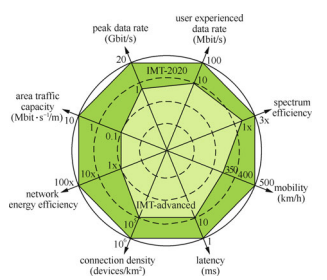
\includegraphics[width=3.5in]{req_pot5G.png}
\caption{Requisitos e Potenciais do 5G \cite{MetisD28}}
\label{req_pot5G}
\end{figure}

\par Em números, esses cenários se traduzem em 100 vezes mais velocidade, crescimento de 10 a 100 vezes do tráfego de informações e  do número equipamentos conectados \cite{METIS3}, somados ao desafio de garantir 5 vezes menos latência e uma duração de bateria 10 vezes maior \cite{Afif}.    
\par As tecnologias disponíveis até a 4G não suportam todas essas funcionalidades ocorrendo simultaneamente. É nesse sentido que se desenvolve a 5G; buscando novas ideias - ou aplicações de ideias antigas de forma inovadora - para possibilitar esta revolução. 
\par  Como foi dito no capítulo introdutório, as possíveis soluções são muitas: \cite{Monserrat} redes de acesso de rádio (RAN) dinâmicas e densas, ferramentas de otimização de uso do espectro, sistema \textit{MIMO} (múltiplas entradas e múltiplas saídas) massivo, diminuição da quantidade de dados dedicada a sinalização e controle, tráfego localizado e interface aérea flexível, opção em que se foca nesta dissertação. 
\par Viu-se que os requisitos de ortogonalidade e sincronismo da geração atual esbarram nas aplicações imaginadas para o futuro. Levando isso em consideração a tecnologia utilizada na camada física deve ser mais flexível. A seção a seguir traz a visão de pesquisadores ao redor do mundo a respeito da utilização de formas de onda alternativas e mostra os possíveis obstáculos a esta opção. 

\section{Formas de Onda Candidatas} 

Em \cite{Maziar}, destaca-se a importância da escolha de uma forma de onda e de um tipo de modulação adequados. Evidencia-se que isto pode trazer impacto ao \textit{throughput} do sistema, à sua confiabilidade e também definir o quão complexo ele será. 
Neste mesmo artigo \cite{Maziar}, são apresentadas as formas de onda candidatas de mais destaque na literatura e como elas conversam com as aplicações e requisitos idealizados para a próxima geração. Estas são categorizadas em formas de onda OFDM e formas de onda FBMC.  

\begin{enumerate}
\item{OFDM}
\par A referência \cite{Maziar} destaca a compatibilidade dos sistemas deste tipo com a técnica MIMO e mostra como cada uma de suas variações podem compensar as características OFDM que são vistas como obstáculos:
\begin{enumerate}
\item{F-OFDM} - (\textit{filtered OFDM}): procura compensar a irradiação para fora da banda mantendo ortogonalidade no domínio do tempo \cite{AbdoliJ}.
\item{W-OFDM} - (\textit{windowed OFDM}): os filtros são aplicados no domínio do tempo e não na frequência (janelamento). Tem-se flexibilidade na escolha da janela, podendo-se optar por uma forma ou outra a depender da aplicação requerida. A vantagem de menos irradiação da F-OFDM é adquirida aqui também. \cite{Maziar}
\item{UF-OFDM} - (\textit{universal filtered OFDM}): a ideia desta forma de onda é filtrar subportadoras em blocos. Além do controle de irradiação observado nas opções anteriores, o UF-OFDM permite tamanhos de quadros variáveis, flexibilizando a largura de banda de cada símbolo, algo muito interessante quando da necessidade de um sistema adaptativo. \cite{Maziar}
\end{enumerate}

\item{FBMC}
\par O FBMC foi construído para oferecer eficiência espectral desde sua concepção. Este alcança tal objetivo filtrando cada sub-portadora que o compõe, mantendo-as bem localizadas no tempo e na frequência \cite{Bellanger}. Suas vantagens são explicitadas em \cite{Maziar}: 
\begin{itemize}
\item redução do \textit{overhead} e da banda de guarda em relação ao OFDM
\item manutenção de desempenho em canais de multi-percurso, mesmo sem prefixo cíclico (CP)
\item atratividade em aplicações assíncronas 
\item possibilidade de manutenção da (semi-)ortogonalidade quando da adoção do O-QAM (\textit{orthogonal quadrature amplitude modulation}) 
\end{itemize}
\end{enumerate}

A maioria dos textos comparativos dessas formas de onda costuma avaliar o desempenho do OFDM em sua forma pura, como desenhado para 4G, e o compara ao FBMC e ao UFMC (\textit{univeral filtered multicarrier}). Esta última tecnologia é uma variação do UF-OFDM, que é mais flexível por permitir o uso de pulsos não retangulares. Aqui, será feito o mesmo tipo comparativo.

\section{Comparação entre Formas de Onda 5G}

Esta seção traz o resultado de algumas análises comparativas de desempenho das formas de onda candidatas à 5G. São observados diferentes cenários, como se vê a seguir: 

\begin{enumerate} 
\item \textbf{Eficiência espectral, Densidade espectral de potência (DPS) e PAPR} \label{irradiação} no contexto aboradado aqui, é começar a falar sobre irradiação para fora da banda (OOB). Sua mitigação é vantajosa em sistemas que exigem sincronismo a medida em que reduzir o "vazamento" espectral evita intereferência entre sub-portadoras adjacentes \cite{YinshengLiu}. Observa-se que, em relação ao OFDM, as formas de onda FBMC e UFMC possuem uma densidade espectral de potência| (DSP) mais concentrada na frequência central \cite{YinshengLiu}, o que mostra que estes sistemas podem apresentar resultados melhores em cenários onde haja desvio de frequência, por exemplo. Em relação a eficiência espectral, \cite{Gerzaguet} mostra que o FBMC ganha eficiência espectral a medida que a duração de quadro aumenta. UFMC por sua vez, supera o OFDM independente disto. Por fim, em relação a PAPR, o FBMC é a forma de onda de melhor desempenho, seguido pelo UFMC. É importante salientar que a diferença é pequena, não ultrapassando os 0.5 dB. \cite{Gerzaguet} 

\item \textbf{Taxa de Erro de Bloco (BLER)} \label{BLER}
\begin{enumerate}
\item \textbf{BLER x SNR} - A comparação entre as três formas de onda, OFDM, FBMC e UFMC mostra que, em termos de taxa de erros, a tecnologia mais robusta é o OFDM \cite{YinshengLiu} \cite{}. Isso já era esperado, visto que a utilização de filtros por si só introduz interferência entre símbolos (ISI). Quanto maior a ordem da modulação utilizada, mais degradado será o desempenho, sendo a UFMC a pior das candidatas neste quesito \cite{YinshengLiu}. 
\item \textbf{Resistência a \textit{offsets} de frequência} - desvios de frequência (CFO) tendem a causar interferência entre subportadoras (ICI). Para avaliar a resposta das formas a este incoveniente, Liu estabelece em \cite{YinshengLiu} que será analisado o comportamento da BLER a medida que a CFO cresce para diferentes valores de SNR. Observa-se uma degradação do resultado quanto maior o CFO, o que era esperado. Nota-se, também, que quanto maior for este parâmetro, menor será o impacto da SNR, visto que a ICI supera a ISI neste caso \cite{YinshengLiu}. Em relação a esta avaliação, a FBMC foi a forma de onda que apresentou melhor desempenho, devido a boa localização no domínio da frequência obtida a partir da filtragem adequada das subportadoras \cite{Boroujeny}. 	
\item \textbf{Mobilidade} - uma das promessas do 5G é o \textit{"amazingly fast"}. Para obtê-lo é necessário ter um desempenho robusto em altas velocidades. O efeito Doppler é capaz de medir este impacto e em \cite{YinshengLiu} mostra-se que a BLER FBMC supera em muito pouco o desempenho das outras duas. 
\end{enumerate}

\item \textbf{Requisitos de Latência} -  Os requisitos de latência exigem boa localização no domínio do tempo. Para este parâmetro, OFDM e UFMC tem um comportamento similar, enquanto o FBMC sofre maior degradação devido a longa resposta ao impulso de seus filtros \cite{YinshengLiu}. 

\item \textbf{Esquema de múltiplo acesso} - na introdução deste capítulo, viu-se o quanto a comunicação assíncrona é importante no contexto do 5G. É por isso que é importante avaliar como essas formas de onda funcionam em um cenário com múltiplos usuários. Em \cite{Gerzaguet} faz-se essa análise em diferentes condições, obtendo-se os seguintes resultados:
\begin{itemize}
\item \textbf{sem banda de guarda e sem desvio de frequência} - considerando o erro de atraso, o FBMC tem a melhor resposta, mas supera em poucos dB o resultado do UFMC e do FBMC
\item \textbf{sem banda de guarda e com 10\% de desvio de frequência} - o comporamento das três formas de onda é bastante similar, sendo o FBMC aquele que supera as outras de forma marginal.
\item \textbf{com 1 portadora de guarda e sem desvio de frequência} - o FBMC supera as outras formas de onda em 40 dB. O UFMC fica em segundo lugar, mas com comportamento muito próximo ao do OFDM.
\item \textbf{com 1 portadora de guarda e com 10\% de desvio de frequência} - o comportamento das formas de onda é similar ao caso anterior.
\end{itemize} 

\item \textbf{Complexidade Computacional} - \label{complexidade} A aplicação de filtros aumenta a complexidade de implementação das formas de onda FBMC e UFMC em relação ao OFDM. Tendo isso em consideração, é necessário confirmar que o impacto não é tão grande a ponto de comprometer outras características, por exemplo a eficiência energética da interface aérea. Em \cite{Eeckhaute} observa-se que o FBMC é menos complexo que o UFMC, que por sua vez exije 100 vezes mais multiplicações que o OFDM para o mesmo número de subportadoras. As equações são mostradas a seguir:
\begin{enumerate}
\item OFDM 
\begin{equation}
C_{OFDM} = n_{b}[2Nlog_{2}N + 4N]
\end{equation}
\item FBMC
\begin{equation}
C_{FBMC} = 2n_{b}[2KN + Nlog_{2}N] + 8n_{b}(2K-1)N 
\end{equation}
\item UFMC
\begin{equation}
\begin{split} 
C_{UFMC} = n_{b}[2Nlog_{2}2N + B(N_{ifft}log_{2}N_{ifft} + 2N_{ifft}log_{2}N_{ifft} + 4\times2N_{ifft}) \\ 
+ 2Nlog_{2}2N + 4N] 	
\end{split}
\end{equation}
\end{enumerate}

\item \textbf{Resposta a amplificadores não lineares}\label{nonlinear}
A resposta de um sistema a não linearidades pode resultar em alargamento espectral, o que como já foi visto, é extremamente prejudicial, principalmente em um cenário MTC (\textit{machine type communications}) \cite{YinshengLi}. Dentre as métricas utilizadas para medir a sensitividade de um sinal a não-linearidades, pode-se citar a PAPR (razão entre a potência de pico e a potência média), e o \textit{backoff}  de potência.
Levando-se esses dois parâmetros em condideração, \cite{Eeckhaute} mostra que, as três formas de onda possuem um comportamento bastante similar, sendo que o UFMC sofre um pouco mais deste efeito que as outras duas. Em relação ao \textit{backoff}, o pior desempenho é observado no OFDM; FBMC e UFMC tem uma resposta bastante similar, em que há pouco alargamento espectral, reduzindo a possibilidade de interferência a subportadoras adjacentes 
\end{enumerate}

O tópico \ref{nonlinear} é muito importante pois trata de uma imperfeição muito comum na transmissão RF. Qualquer sistema faz uso de amplificadores, usualmente não-lineares. A mitigação deste efeito é bastante complexa e este tópicos ainda pode ser bastante explorado no contexto da 5G. A seção a seguir apresenta as conclusões a que chegaram alguns autores a respeito de mecanismos de correção. 

\section{Mecanismos de Correção de Não Linearidades}

O mecanismo mais popular para a correção de não linearidades no âmbito do 4G é a pré-distorção digital (DPD). O algortimo foi aplicado para compensar não linearidades em ambiente MIMO \cite{gregorio}, em comunicações via fibra-óptica \cite{Shang}, \cite{Silva} e também levando-se em consideração a transmissão OFDM num contexto de agilidade espectral, semelhante ao que vai ser visto na 5G \cite{ZhuFu}. 
\par O algoritmo consiste em um mecanismo de feedback, em que algumas iterações são realizadas até que se obtenha o resultado ótimo. Observa-se que a cada \textit{loop}, tem-se um uma redução de mais de 20dB na DSP que está fora da banda \cite{ZhuFu}, o que se traduz em um desemepenho mais robusto em termos de BER (taxa de erro de bit), já que a ICI será muito menor. 
\par Esses resultados chamam a atenção para a efetividade do algortimo e despertam o interesse de aplica-lo, também às formas de onda da 5a geração.Em \cite{Zhang}, a metodologia é aplicada transmissores 5G, mas não há nenhum destaque a forma de onda utilizada na camada PHY e nenhuma análise comparativa entre as candidatas. Em \cite{Abdelaziz}, traz-se a resposta do FBMC a DPD, comparando o desempenho ao OFDM, porém não faz menção ao comportamento da UFMC. 
\par Essa carência de textos que tratem da correção de não-linearidades, aponta para a necessidade de um maior número de estudos a respeito deste tema. Nessa dissertação, procura-se reduzir esta lacuna. O capítulo 5 traz uma análise comparativa da resposta das três formas de onda ao algoritmo DPD para diferentes tipos de modulação digital. De forma complementar, apresenta-se, também o resultado da aplicação de um algoritmo de correção chamado ICDH (\text{iterative correction with hard detection}), que será descrito em momento oportuno e finalmente, mostra-se o quanto a codificação pode ajudar na correção de não linearidades, avaliando-se qual metodologia é mais vantajosa. 




